
\documentclass{pnastwo}
\usepackage{graphicx}
\usepackage{amsmath}
\usepackage{lscape}
\newcommand{\xline}[0]{\noindent\underline{\makebox[0.15cm][l]{}}}
\makeatletter
\def\hlinewd#1{%
	\noalign{\ifnum0=`}\fi\hrule \@height #1 \futurelet
	\reserved@a\@xhline}
\makeatother
\begin{document}
	
	
\title{The relationship between scaled selection coefficients and dN/dS}
	
\author{Stephanie J. Spielman\affil{1}{Department of Integrative Biology, Center for Computational Biology and Bioinformatics, and Institute of Cellular and Molecular Biology.
		The University of Texas at Austin, Austin, TX 78712, USA.} 
	\and
	Claus O. Wilke\affil{1}{}
}
	
\contributor{Submitted to Proceedings of the National Academy of Sciences of the United States of America}
\maketitle

\begin{article}
		
\begin{abstract} %PNAS - 250 words. We are currently at 260, but probably this whole abstract is trash :) 
Two broad classes of Markov-process models have been developed to describe the strength of natural selection in protein-coding sequences in a phylogenetic context. The first and most widely-used modeling framework estimates the evolutionary rate ratio $dN/dS$, which represents the ratio of nonsynonymous to synonymous substitution rates, in a maximum likelihood (ML) framework. These models have been developed to a high level of sophistication and are a staple of modern-day comparative sequence analysis. The second class of models, known as mutation-selection-balance (MutSel) models, explicitly consider the dynamic interplay between mutation and selection. Instead of $dN/dS$ estimates, these models calculate site-specific amino-acid and/or codon scaled selection coefficients, which indicate the extent to which natural selection acts on all possible mutations. However, the extent to which these two modeling frameworks relate to each other is unknown. Do $dN/dS$ estimates reveal similar or distinct information from scaled selection coefficients? To answer this question, we derive a formal mathematical relationship between these two quantities. We find that scaled selection coefficients can  precisely predict $dN/dS$, indicating that $dN/dS$ and MutSel models \textbf{are in complete agreement}. We additionally show that $dN/dS$ calculated from selection coefficients is strictly less than 1, and thus MutSel models inherently cannot describe positive selection and/or adaptive evolution. However, if synonymous mutations are not neutral, it is actually possible for $dN/dS$ to be greater than 1, even though positive selection is not occurring. Finally, we find that ML $dN/dS$ models produce systematically biased $dN/dS$ estimates when nucleotide mutation rates are asymmetric, demonstrating that these models do not properly account for nucleotide compositional bias.
\end{abstract}
		
\keywords{dN/dS | mutation-selection-balance models | scaled selection coefficients | Markov models of sequence evolution}
		
\section*{Introduction}
		
The oldest and most-widely used method to infer selection pressure in protein-coding genes calculates the evolutionary rate ratio $dN/dS$, which represents the ratio of non-synonymous to synonymous substitution rates. This metric indicates how quickly a protein's constituent amino acids change, and it is commonly used to identify proteins or protein sites that experience negative selection ($dN/dS<1$), evolve neutrally ($dN/dS\approx1$), or experience positive, diversifying selection ($dN/dS>1$) \cite{NielsenYang1998, Yangetal2000, KosakovskyPondFrost2005b, Huelsenbecketal2006}. Frameworks for calculating $dN/dS$ have broadly fallen into two camps: heuristic counting methods \cite{LWL85,NG86,Pamilo1993,Ina1995,YN00} and maximum likelihood (ML) methods \cite{GoldmanYang1994,MuseGaut1994,NielsenYang1998,Yang2006}. The latter variety assume an explicit Markov-process model of sequence evolution to yield maximum likelihood estimates (MLEs) of the parameter $\omega$, which represents the quantity $dN/dS$ (although we note that other styles of these models use separate parameters for nonsynonymous and synonymous substitution rates \cite{MuseGaut1994,KosakovskyPondMuse2005}). These $dN/dS$ models have become a staple of comparative sequence analysis since their introduction in the 1990s (see ref \cite{Anisimova2009} for a comprehensive review), and we will refer to them as $\omega$ models throughout this paper.

A second class of models, known as mutation-selection-balance (MutSel) models, are increasingly being viewed as a viable alternative to $\omega$ models. While $\omega$ models describe the how quickly a protein's constituent amino acids change, MutSel models assess the strength of natural selection operating on specific amino-acid or codon changes. In particular, the MutSel framework, couched firmly in population genetics theory, considers the specific selective responses to of all site-wise mutations in a protein-coding sequence \cite{HalpernBruno1998,Thorne2012}. MutSel models yield estimates of site-wise scaled selection coefficients $S=2N_es$, which indicate the extent to which natural selection favors, or disfavors, particular codon or amino acid changes \cite{HalpernBruno1998,YangNielsen2008,Rodrigueetal2010,Tamurietal2012}. Although first introduced over 15 years ago \cite{HalpernBruno1998}, MutSel models have seen little use due to their high computational expense. Recently, however, several computationally tractable model implementations have emerged \cite{RodrigueLartillot2014,Tamurietal2014}, allowing for the first time the potential for widespread adoption.		
		
$\omega$ models have undergone rigorous development in their 20 years of existence and have advanced to high levels of sophistication. These models can accommodate a variety of evolutionary scenarios, including synonymous rate variation \cite{MuseGaut1994,KosakovskyPondMuse2005}, episodic \cite{KosakovskyPondetal2011,MEME} and/or lineage-specific selection \cite{YangNielsen2002,Zhangetal2005,KosakovskyPondFrost2005a}, and they can also incorporate information regarding protein structure and/or epistatic interactions \cite{Robinsonetal2003,Thorneetal2007,Rodrigueetal2009,Scherreretal2012,MeyerWilke2012}. This flexibility, along with accessible software implementations \cite{KosakovskyPondetal2005,Yang2007,Delport2010}, make $\omega$ models a very attractive modeling choice. On the other hand, some have argued that MutSel models, given their explicit consideration of population genetics theory and attention to site-specific amino acid fitness differences, offer a more fine-grained approach to studying protein evolution than do $dN/dS$ models \cite{HalpernBruno1998,Rodrigueetal2010,Tamurietal2012,Thorne2012}. Recent phylogenetic studies have also demonstrated that evolutionary models which account for amino acid fitness values dramatically outperform other $\omega$ models, suggesting that MutSel models may more aptly represent the evolutionary process \cite{Bloom2014a, Bloom2014b}. 
		
Although both $\omega$ and MutSel models describe the same fundamental process of protein-coding sequence evolution along a phylogeny, it is unknown how these two modeling classes relate to one another. In particular, as these inference methods have been developed independently, it remains an open question whether or not parameter estimates from one model are comparable to those of the other model. As a consequence, although certain rhetorical arguments may be made in favor of using one method over another, there is currently no formalized, concrete rationale to guide researchers in their methodological choices. Elucidating the relationship between these competing modeling frameworks will more precisely reveal under which circumstances the use of these models is justified.
		
Here, we formalize the relationship between $\omega$ and MutSel models by examining the extent to which their respective focal parameters, $dN/dS$ and scaled selection coefficients, yield overlapping information about the evolutionary process. To this end, we derive a mathematical framework to calculate $dN/dS$ values from scaled selection coefficients. We find that $dN/dS$ values can be precisely calculated from scaled selection coefficients, and that $dN/dS$ and the distribution of scaled selection coefficients are strongly related. Furthermore, we prove that, when synonymous mutations are neutral, $dN/dS$ calculated from selection coefficients is necessarily less than 1. This proof demonstrates that MutSel models are inherently only able to model purifying selection, and therefore would be an inappropriate model choice if positive selection is expected. However, we also find that, when synonymous codons have different fitnesses, it is possible to recover $dN/dS$ values above 1, even though no positive selection is occurring. 

Finally, we are able to use this robust relationship to assess the performance of $\omega$ models. If $\omega$ models are behaving as expected, we expect that they will yield the same $dN/dS$ estimates as our calculations. We find that, in the absence of nucleotide compositional bias, $dN/dS$ values inferred in an ML framework agree precisely with those calculated from scaled selection coefficients, meaning that MutSel and $dN/dS$ models are in complete agreement. However, we found that, in the presence of mutational or nucleotide biases, ML inference frameworks produce systematically biased $dN/dS$ estimates. 
		
		
\section*{Results and Discussion}
		
		
\subsection*{Theoretical model.}

We model sequence evolution as a continuous-time Markov process \cite{Yang2006} under the assumptions of a fixed effective population size $N_e$ and constant selection pressure over time. This process is governed by the $61 \times 61$ transition matrix $P(t) = e^{Qt}$, where the corresponding instantaneous rate matrix $Q$ gives the instantaneous substitution probabilities between all 61 sense codons. We further assume that only single nucleotide changes occur instantaneously. We adopt the Halpern-Bruno \cite{HalpernBruno1998,YangNielsen2008,Tamurietal2012,Thorne2012} MutSel modeling framework, which models the evolutionary process with explicit population genetics theory. 

To being, let $f_i$ be the fitness of codon $i$, and thus the selection coefficient acting on a mutation from codon $i$ to codon $j$ is $s_{ij} = f_j - f_i$ \cite{SellaHirsh2005,YangNielsen2008}. The fixation probability for a mutation from codon $i$ to codon $j$ is given by 
\begin{equation}\label{eq:u_ij}
u_{ij} = \frac{2s_{ij}}{1 - e^{-2N_es_{ij}}} \approx \frac{1}{N_e}\frac{2N_es_{ij}}{1 - e^{-2N_es_{ij}}}
\end{equation} \cite{Kimura1962,HalpernBruno1998,YangNielsen2008}. 

We further define $S_{ij} = 2N_es_{ij}$ as the scaled selection coefficient for this mutation. We model the substitution as the product of fixation and mutation rates, $\mu$. 

Therefore, the substitution probability for codon $i$ to codon $j$ is 
\begin{equation}\label{eq:q_ij}
q_{ij} = N_e\mu_{ij}u_{ij} = \mu_{ij}\frac{S_{ij}}{1 - e^{-S_{ij}}} , 
\end{equation} and this expression corresponds to the instantaneous matrix element $Q_{ji}$. 
\cite{HalpernBruno1998,SellaHirsh2005}. 

Given detailed balance (reversibility), we have 
\begin{equation}\label{eq:DB}
q_{ij}P_i = q_{ji}P_j,
\end{equation} 
where $P_i$ is the stationary frequency of codon $i$. 

From equations \eqref{eq:q_ij} and \eqref{eq:DB}, we can write the ratio of substitution probabilities as 
\begin{equation}\label{ratio_q_ij}
\frac{q_{ij}}{q_{ji}} = \frac{P_i \mu_{ij} S_{ij} (1-e^{-S_{ji}})}{P_j \mu_{ji} S_{ji} (1-e^{-S_{ij}})} 
\end{equation}


Given that $S_{ij} = -S_{ji}$, we can simplify equation \eqref{ratio_q_ij} to show that $q_{ij}/q_{ji} = e^{S_{ij}}$, and we therefore find that
\begin{equation}\label{eq:s_pmu}
S_{ij} = \ln\bigg{(} \frac{P_j\mu_{ji}}{P_i\mu_{ij}} \bigg{)}. 
\end{equation}
These equations establish a relationship between scaled selection coefficients and the stationary codon frequencies of the Markov model. Moreover, we note that in the specific case of symmetric mutation rates $\mu_{ij} = \mu_{ji}$, we have $S_{ij} = \ln\big{(}{\frac{P_j} {P_i}}\big{)}$ \cite{SellaHirsh2005}. 


		
\subsection*{Mathematical relationship between scaled selection coefficients and dN/dS.} 

Using the theory laid out in the previous subsection, we can calculate an evolutionary rate by summing over all substitution probabilities weighted by the frequency of the originating codon. Further, we can establish specific expressions for nonsynonymous and synonymous evolutionary rates, and then divide them in order to obtain a value for the evolutionary rate ratio $dN/dS$.

To begin, we can write the nonsynonymous rate $K_\text{N}$ as 
\begin{equation}\label{eq:KN}
	K_\text{N} = N_e \sum_i \sum_{j \in {\cal N}_i} P_i \mu_{ij} u_{ij} \,,
\end{equation}
where ${\cal N}_i$ is the set of codons that are nonsynonymous to codon $i$ and differ from it by one nucleotide. To normalize $K_\text{N}$, we divide it by the number of nonsynonymous sites, which we calculate according to the mutational opportunity definition of a site \cite{GoldmanYang1994, Yang2006} as 
\begin{equation}\label{eq:LN}
	L_\text{N} = \sum_i \sum_{j \in {\cal N}_i} P_i \mu_{ij}\,, 
\end{equation} and thus we find that 
\begin{equation}\label{eq:dN}
	dN = \frac{K_\text{N}}{L_\text{N}}=\frac{N_e \sum_i \sum_{j \in {\cal N}_i} P_i \mu_{ij} u_{ij} } {\sum_i \sum_{j \in {\cal N}_i}P_i \mu_{ij}}\,.
\end{equation}
		
Similarly, for $dS$, the synonymous evolutionary rate $K_\text{S}$ per synonymous site $L_\text{S}$, we have
\begin{equation}\label{eq:dS}
	dS = \frac{K_\text{S}}{L_\text{S}}=\frac{ N_e \sum_i \sum_{j \in {\cal S}_i} P_i \mu_{ij} u_{ij} } {\sum_i \sum_{j \in {\cal S}_i} P_i \mu_{ij} }\,,
\end{equation}
where ${\cal S}_i$ is the set of codons that are synonymous to codon $i$ and differ from it by one nucleotide substitution. The quantities $K_\text{S}$ and $L_\text{S}$ are defined as in Eqs.~\eqref{eq:KN} and \eqref{eq:LN} but sum over $j\in {\cal S}_i$ instead of $j\in {\cal N}_i$. Moreover, we note that, if we make the dual assumptions that nucleotide mutation rates are symmetric and that all synonymous codons have equal fitness (i.e.\ synonymous mutations are neutral), the synonymous fixation rate $u_{ij}= 1/N_e$ \cite{CrowKimura1970}. Under this circumstance, the value for $dS$ reduces to 1.
		
				
\subsection*{dN/dS accurately reflects selection strength.}

Using the theoretical framework established in equations \eqref{eq:u_ij} - \eqref{eq:dS}, we can examine the relationship between the $dN/dS$ values corresponding to different distributions of scaled selection coefficients. To this end, we generated 200 distinct distributions of amino acid fitness values $f_a$. We drew these 20 amino acid fitness values from a normal distribution $\mathcal{N}(0,\sigma^2)$, where $\sigma^2 \sim \mathcal{U}(0,4)$. Here, $\sigma^2$ effectively represents the strength of natural selection; higher $\sigma^2$ correspond to larger fitness difference among amino acids, prompting selection to act more strongly against nonsynonymous changes. In other words, high $\sigma^2$ values indicate strong purifying selection, while lower values indicate weaker purifying selection. We additionally note that these amino acid fitness quantities correspond to the amino acid propensity parameters estimated by currently available MutSel inference methods \cite{RodrigueLartillot2014,Tamurietal2014}.

We then converted each distribution of amino acid fitnesses to a corresponding set of codon fitnesses. For 100 of the distributions, we assumed that synonymous changes were neutral, and thus we directly assigned each codon the same fitness $f_i = f_a$. For the other 100 sets of fitnesses, we allowed synonymous codons to have different fitness values. In these circumstances, we randomly selected a preferred codon for each amino acid, and we assigned the preferred codon the fitness of $f_i = f_a + \lambda$ and all non-preferred codons the fitness $f_i = f_a - \lambda$. We drew a unique $\lambda$ for each fitness distribution from $\mathcal{U}[0,2]$. We refer to first set of codon selection coefficients as ``no codon bias," and the second set as ``codon bias." 

Finally, using equations \eqref{eq:u_ij} - \eqref{eq:dS}, we computed $dN/dS$ for each distribution of codon fitnesses. For these calculations, we also need to select mutation rates. We set the mutation rate for transitions as $\mu\kappa$, and the rate for all transversions as $\mu$. We use the value $\mu = 10^{-6}$ for all $dN/dS$ calculations, and we draw a unique value for $\kappa$ from $\mathcal{U}[1,6]$ for each set of codon fitnesses.

We found that $dN/dS$ values scale excellently with the variance ($\sigma^2$) of the distribution of amino-acid scaled selection coefficients (Figure~\ref{dnds_variance}). As Figure~\ref{dnds_variance} shows, $dN/dS$ and $\sigma^2$ are strongly negatively correlated; when fitness differences among amino acids are very high, $dN/dS$ takes on lower values, properly reflecting stronger purifying selection. Furthermore, as expected, this trend is much stronger for alignments without codon bias (Figure~\ref{dnds_variance}A, $r^2 = 0.83$) than for alignments with codon bias (Figure~\ref{dnds_variance}B, $r^2 = 0.45$). The weakened relationship for alignments with codon bias emerges from the fact that fitness differences among synonymous codons will obscure underlying amino acid fitness differences. Even so, the presence of codon bias does not remove the significant negative correlation between $dN/dS$ and selection strength.
		
Importantly, Figure~\ref{dnds_variance}A demonstrates that, in the limiting case when $\sigma^2$ approaches 0, and thus all codons have virtually the same fitness, $dN/dS$ converges to 1. More precisely, the largest $dN/dS$ value recovered for alignments without codon bias was 0.997, and this alignment featured a $\sigma^2 = 0.08$. This result properly reflects the case of neutral evolution. In fact, in \textbf{PROOF}, we prove that, when synonymous changes are neutral and mutation is symmetric (i.e.\ $\mu_{xy} = \mu_{yx}$), $dN/dS$ is necessarily always less than or equal to 1. We have also proven that, when synonymous changes are neutral and mutation rates are symmetric, $dN/dS$ as calculated from scaled selection coefficients will always be less than 1. This proof formalizes the MutSel model underlying assumption that selection pressure is constant over the phylogeny and confirms that MutSel models are inherently unable to describe positive, diversifying selection. Although this proof assumes symmetric nucleotide mutation rates, we do not expect that deviations from this assumption will have dramatic effects on $dN/dS$ estimates. Therefore, we conclude that the MutSel framework is an inappropriate model when positive selection is expected, as the model may yield spurious and misleading results. 

However, this restriction of $dN/dS < 1$ does not hold when synonymous changes are not neutral, as seen in Figure~\ref{dnds_variance}B. In other words, even though the underlying evolutionary model assumes evolutionary equilibrium, i.e.\ selection pressures remain constant over time and hence there is no positive, diversifying selection, $dN/dS$ can readily be greater than 1. Indeed, it is theoretically possible to achieve arbitrarily high $dN/dS$ values when there are fitness differences among synonymous codons; in the most extreme case of codon bias, where only a single codon per amino acid is selectively tolerated, the number of synonymous sites $L_\text{S} = 0$, and thus the value for $dN/dS$ approaches infinity. Given that the MutSel model framework assumes an overarching regime of purifying selection, this finding might seem paradoxical. However, the logical argument that $dN/dS > 1$ represents positive, diversifying selection assumes that the rate of synonymous change may be used as a neutral benchmark, an assumption which codon bias clearly violates. Thus, in theory, what is classically termed positive selection can result simply from strong synonymous fitness differences. 	
		
We acknowledge that it is unlikely that this result will have a strong influence in real analyses, as selection on synonymous codons is likely relatively weak in most taxa \cite{HershbergPetrov2008}. For instance, experimental evidence from the yeast Hsp90 protein suggests that, while there are some fitness differences among synonymous codons, these differences are exceedingly minimal compared to fitness differences among amino acids \cite{Hietpas2011,Hietpas2013}. Moreover, our implementation of codon bias explicitly assumed that selection alone, and not mutation, was the sole source of codon bias. This implementation might not be entirely biologically realistic, as both mutational and selective forces likely contribute to codon bias in real genomes \cite{Blumer1991, Duret2002, HershbergPetrov2008, Chen2009, PlotkinKudla2010}. Even so, the fact that $dN/dS$ can theoretically bear the hallmark of positive selection, even when purifying selection alone is occurring, is an important insight. It is, therefore, possible that estimates of positive selection in species with high levels of codon bias driven in part by selection, such as bacterial, \textit{Drosophila}, or certain mammalian species \cite{Duret2002, Chamaryetal2006, PlotkinKudla2010}, may not be true cases of positive selection, but rather signals of strong codon bias. 

\subsection*{dN/dS calculated from ssc's as a model benchmark.}

As a consequence of the relationship between $dN/dS$ and scaled selection coefficients, we have a unique opportunity to assess the robustness of $dN/dS$ inference methods. It is conventional practice in model development to benchmark the model against data simulated according to the model itself. While this strategy is crucial for testing whether a model was implemented correctly, it is inherently incapable of discerning limitations and properties of the inference framework under more general conditions. Moreover, it cannot confirm that the underlying model accurately represents the evolutionary process. Therefore, we apply a novel benchmarking approach which uses the theoretical relationship among modeling frameworks to assess the accuracy and specific utility of those models. This approach, outlined in Figure~\ref{reg_conv}A, entails comparing $dN/dS$ values calculated from selection coefficients to those inferred by an $\omega$-based model, in order to benchmark the model's accuracy.

Using the selection coefficients and mutation rates derived in the previous subsection, we simulated alignments using standard methods \cite{Yang2006} according the Halpern-Bruno MutSel model \cite{HalpernBruno1998}. We then inferred $dN/dS$ for each alignment using the M0 model \cite{GoldmanYang1994,Yangetal2000}, as implemented in the HyPhy batch language \cite{KosakovskyPondetal2005}. This model uses the GY94 instantaneous rate matrix, which includes parameters for transition/transversion bias ($\kappa$), equilibrium codon frequencies ($\pi$), and finally the $dN/dS$ rate ratio ($\omega$) (see equation \eqref{eq:GY94}). Throughout the remaining text, we refer to $dN/dS$ as inferred by M0 as $\omega$, and to $dN/dS$ computed using equations \eqref{eq:u_ij} - \eqref{eq:dS} simply as $dN/dS$. 

We found that $dN/dS$ values agree nearly perfectly with $\omega$ values (Figure~\ref{reg_conv}B). This agreement was neither influenced by the presence of codon bias, nor by nucleotide compostitional bias; indeed, simulated alignments featured a wide range (0.21-0.89) of GC contents. Additionally, in Figure~\ref{reg_conv}C, we demonstrate that $\omega$ converges to the true $dN/dS$ value as the size of the data set, represented by simulated alignment length, increases. These results unequivocally show that the $dN/dS$ quantity is fully contained within MutSel model parameters, and importantly that ML $dN/dS$ inference methods are robust indeed reveal that ML $dN/dS$ inference frameworks behave exactly as expected, yielding precise $dN/dS$ estimates. This finding has important implications for modeling choices; although the MutSel framework might model the sequence evolution in a way that more mechanistically matches the evolutionary process, $\omega$-based models do not dramatically suffer from any modeling limitations. 

\subsection*{dN/dS inference with realistic data.}
Having confirmed that $\omega$-based and MutSel models \textbf{agree} under general conditions, we sought to test the accuracy of $\omega$-based models using more realistic data. To this end, we made use of realistic amino acid fitness and nucleotide mutation rate parameters to construct a series of experimental evolutionary models. In particular, we used influenza nucleoprotein (NP) site-specific amino acid preference values, given by ref. \cite{Bloom2014a}, which consisted of experimentally-determined fitness values for each individual amino acid across all sites in NP, yielding 498 distinct amino acid propensity distributions. We combined these experimental fitness parameters with three sets of experimentally determined mutation rates, either for NP \cite{Bloom2014a}, yeast \cite{Zhu2014}, or polio virus \cite{Acevedo2014}. While each of these mutation matrices is asymmetric, they feature differing degrees of asymmetry, with NP mutation rates being the most symmetric and polio mutation rates the most asymmetric. More precisely, in the absence of amino-acid level selection, the GC contents that the NP, yeast, and polio mutation rates would generate are 0.518, 0.336, and 0.192, respectively. Finally, we built a unique experimentally-informed evolutionary model for all combinations of amino acid fitness distributions and mutation rates using the approach outlined in refs. \cite{Bloom2014a,Bloom2014b}. We calculated stationary codon frequencies for each experimental model, and used these values in combination with their corresponding mutation rates to simulate sequences and infer $dN/dS$ quantities. 


As different M0 model parameterizations are known to yield distinct $\omega$ estimates \cite{ZhangYu2006,Yang2006}, we inferred $\omega$ using the commonly-used frequency estimators F61 \cite{GoldmanYang1994}, F3x4 \cite{MuseGaut1994}, and CF3x4 \cite{Pond2010}. The F61 estimator approximates these model parameters using an alignment's empirical codon frequencies, while the F3x4 and CF3x4 estimators approximate codon frequency parameters using positional nucleotide frequencies. We calculated values for codon frequency parameters using two different ways. First, we used the empirical codon frequencies found in the simulated alignments; as we simulated unique alignments for all site-specific amino acid preferences, we pooled all alignments for a given mutation rate specification to determine the global empirical frequencies, and subsequently calculate values for F61, F3x4 and CF3x4 frequency parameterizations. This strategy is analogous to how these frequency parameters are estimated in common practice. Second, we computed frequency parameter values using the codon frequencies which would exist in the absence of natural selection, but would arise strictly from mutational processes. As these values correspond precisely to those intended for these model parameters \cite{GoldmanYang1994,MuseGaut1994,YN00,Yang2006}, we term these the ``True Frequencies."

Overall, we found that $\omega$-based models clearly before best when mutation rates symmetric.

We found that these results, while still pretty good, were not as good as under symmetric mutation rates. NP, which is the closest to symmetric, yielded very good results, with high correlations and minimal bias. On the other hand, yeast and polio go nuts. Presence of asymmetric mutation rates led all M0 model parameterizations to systematically infer underestimated values. 
We found that the three frequency estimators performed comparably, $\omega$ estimates are systematically biased downwards as mutation rates become increasingly asymmetric. This trend generally holds regardless of the frequency estimator used (with a single exception, which we discuss below). $\omega$ inferences on alignments with NP mutation rates have the least amount of bias, followed by yeast and finally polio mutation rates, and a parallel trend exists for the correlation strengths. However, using true frequencies (Figure~\ref{nyp_bias_r2}C-D), as opposed to empirical (Figure~\ref{nyp_bias_r2}A-B) frequencies, did reduce the bias (mean absolute decrease of 4.47\%)for simulations which used polio mutation rates, but bias was largely unchanged for NP and yeast mutation rates. Additionally, correlations between $\omega$ and $dN/dS$ were generally higher when empirical frequencies were used instead of true frequencies. Taken together, these results suggest that current codon frequency estimators cannot fully account for strongly asymmetric mutation rates and/or even nucleotide composition introduced by mutation. 

Therefore, we sought to ameliorate this systematic bias by introducing a novel model parameterization, which we term ``Fnuc." Fnuc merges the equilibrium nucleotide and codon frequencies to reveal a distinct target nucleotide frequency for each specific instantaneous change. Therefore, this parameterization takes into account both mutation at the nucleotide level as well as overarching codon frequencies. A derivation of this parameterization is given in \textbf{Appendix 2}. We used the Fnuc parameterization to again infer $\omega$, using both empirical and true frequencies. We found that Fnuc substantially reduces bias while simultaneously increasing precision in $\omega$ estimates, in particular for the yeast mutation rates. While empirical Fnuc did not dramatically improve bias for the polio mutation rate data set, it did offer improvements over all other frequency estimators. We additionally note that the polio mutation rates were strongly asymmetric, and in the absence of selection would lead to the strongly biased A/T content of roughly 80\%. Thus, we recommend that future implementations of $\omega$-based models consider the Fnuc parameterization, as it has the ability to reduce misleading signal induced by asymmetric mutation rates.

%There is a noteworthy exception to the overall trend of $\omega$ underestimation; $\omega$ MLEs for NP mutation rates, when computed using F61, were actually overestimates of $dN/dS$. We attribute this result to the fact that the NP mutation rates were only minimally asymmetric, and in the absence of natural selection, these mutation rates would produce nearly even nucleotide frequencies. Importantly, when nucleotide mutation rates are symmetric, steady-state codon frequencies are controlled only by selection, as there is no opportunity to generate compositional bias through mutation \cite{SellaHirsh2005}. Therefore, because the F61 estimator directly uses empirical codon frequencies, the resulting M0 codon frequency parameters actually contain information about the strength of natural selection. The end result is that selection pressures which should be strictly incorporated in the $\omega$ parameter are inadvertently contained within the codon frequency parameters. Thus, the model infers selection to be weaker than it actually is, producing elevated $\omega$ MLEs. Although the $\omega$ overestimation was relatively small in this particular case, this example highlights that it is crucial to properly parameterize $\omega$-based models. If these models are incorrectly parameterized, the $\omega$ parameter will no longer accurately represent the $dN/dS$ evolutionary rate ratio, but will instead be a meaningless quantity.



\section*{Future Directions}
		
We will conclude with insights gained from our study and recommendations for using $\omega$-based and MutSel modeling frameworks going forward. We have shown that $dN/dS$ be accurately calculated from selection coefficients, revealing that $\omega$-based and MutSel models yield consistent and overlapping information about the strength natural selection. Importantly, our proof that $dN/dS \leq 1$, when calculated from selection coefficients and when synonymous mutations are neutral, indicates that the use of MutSel models is only justified under conditions of strictly purifying selection, or neutral evolution. This restriction is in part indicated by the basic MutSel model assumption of constant selection pressures over time, or in other words a static fitness landscape \cite{HalpernBruno1998,Thorneetal2007,Rodrigue2010,Thorne2012}. 

Thus, if the aim is to identify positive selection, only $\omega$-based models, of the two frameworks examined here, are justified. However, there are still some theoretical issues with the approach that these models take, namely in their use of equilibrium codon frequency parameters. We expect that, if positive selection is occurring, there is necessarily a shift in the underlying fitness landscape causing different amino acids to become preferred. 





$\omega$-based models are an apt model choice for examining positive, diversifying selection. However, if one desires site-specific point estimates of $dN/dS$, $\omega$-based models   

 
2. if and when you use omega models, you absolutely must parameterize them properly, otherwise dnds is a meaningless quantity. this seems difficult to do. there is an internal tension in omega models, wrt to equilibrium codon frequencies. If codon frequencies are assumed to be at equilibrium, how can we ever properly account for adaptive processes, such as positive selection? moreover, if we screw up any model parameter, dnds may be wrong. suggests that point estimates for dnds from these models are not ideal, see that one plos response. precise point estimates can, however, be calculated from a mutsel model, provided purifying selection. but if detecting positive selection is your goal, seriously do NOT use mutsel models. future work should investigate modeling frameworks which fully account for nonequilibrium evolutionary processes.

We additionally emphasize that improper model parameterizations lead to spurious $\omega$ MLEs which do not accurately represent $dN/dS$. If other model parameters ($\kappa$ and equilibrium codon frequencies) are specified incorrectly, or inadvertently contain information about amino-acid level natural selection, the resulting $\omega$ MLE will not represent the true $dN/dS$ evolutionary rate ratio. Only by ensuring that $\omega$ is the only model parameter which contains information about natural selection will it assuredly represent $dN/dS$. 
		
		Taken together, these results strongly suggest that the MC model's codon frequency parameters are ill-suited to accomodate compositional biases which result from forces other than amino-acid level selection. We therefore suggest that future work investigate the utility of novel parameters for MC models which better account for asymmetry in the mutational process.
		

%Therefore, it appears that, when nucleotide compositional bias results from mutational processes, MC models produce negatively biased $dN/dS$ estimates. MC models attempt to deal with mutation-induced nucleotide compositional bias through the use of equilibrium codon frequency parameters \cite{Yang2006}. Unlike the equilibrium, stationary frequencies on which we have focused throughout this paper, these frequency parameters are intended to represent the codon frequencies which would exist in the absence of amino-acid level selection, but from mutational or other biological processes, such as GC-biased gene conversion \cite{DuretGaltier2009,WebsterHurst2012}, alone \cite{GoldmanYang1994,MuseGaut1994,YN00,Yang2006}. However, even a codon frequency parameterization using precisely these values (Ftrue) still suffers from a decrease in accuracy as mutation-induced nucleotide compositional bias increased. Surprisingly, the Fequal frequency parameterization, which assigns parameter values of $1/61$ for all sense codons and is therefore no different from a matrix-scaling factor, performs just as well, if not better, than do all other frequency parameterizations, including the standard F61, F3x4, and CF3x4 estimators. 
		
		

		
%The $dN/dS$ calculations we have proposed differ fundamentally from previously proposed frameworks, including both counting \cite{LWL85,NG86,Pamilo1993,Ina1995,YN00} and maximum likelihood methods \cite{GoldmanYang1994,MuseGaut1994,Yang2006,Anisimova2009}, in that they are solidly grounded in population genetics theory. Counting methods, on the other hand, simply enumerate the number of nonsynonymous and synonymous changes, weighted by the number of sites, and maximum likelihood methods effectively yield a summary statistic $\omega$ which is expected to equal $dN/dS$. That the $dN/dS$ values calculated using equations \eqref{eq:pi_i} - \eqref{eq:dS} agree precisely with $\omega$ estimates inferred from the M0 model lends firm support for the validity of our $dN/dS$ calculations, and indeed to the methodological accuracy of MC models. We emphasize, however, that our method for computing $dN/dS$ is only suitable when the protein is evolving strictly at equilibrium, or when selection pressures are constant over the phylogeny.
		% % % % % % % % % % NONEQUILIBRIUM AND POSITIVE SELECTION STUFF % % % % % % % % % % %
		% things that our study does not account for - gc bias produced by bias gene conversion. this is likely a selective force that systematically generates compositional bias, but cannot necessarily be accounted for amino acid selection coefficients. In theory, mech codon models incorporate this info via their codon frequency parameters, but mutation-selection models have no such equivalent parameter. possible future efforts could incorporate biases that stem from biological mechanisms other than amino acids and nucleotides.
		
		%This relationship holds only if the protein evolves accordingly to a strictly steady-state process, otherwise known as purifying selection. Alternatively, under non-equilibrium conditions, (e.g. positive selection, when $\omega > 1$), MutSel models are inherently unable to describe protein evolution. These findings have important implications for when the use of each model is justified; if positive selection has occurred along the protein's evolutionary trajectory, MutSel models will likely yield spurious results. This proof, however, only holds when mutation rates are symmetric and when synonymous codons have equal fitnesses. 
		%Our results rest on the key assumption that the protein sequence is evolving under steady-state, or equilibrium, conditions. The assumption exactly recapitulates the population genetics theory behind MutSel models, which assume that selection coefficients remain constant over the phylogeny, and therefore the protein is evolving along a static fitness landscape \cite{HalpernBruno1998,YangNielsen2008,Rodrigueetal2010,Tamurietal2012}. 
		%Positive, diversifying selection is assumed to occur when the protein sequence experiences strong selective pressure to change its constituent amino acids. Positive selection, therefore, necessarily implies that the protein does not evolve at equilibrium, but rather a shift in selective constraint caused new amino acids to be favored. 
		%  $dN/dS$ is used as a hallmark identifier for the three natural selection paradigms of purifying selection ($dN/dS < 1$), neutral evolution ($dN/dS = 1$), and finally positive selection ($dN/dS > 1$). Our analysis revealed that this classical $dN/dS = 1$ threshold might not be universally applicable. Indeed, all simulations presented here relied on the protein evolving under a steady-state process, or in other words, along a static fitness landscape. In a system where selective pressures remain constant along the phylogeny time, we expect purifying selection to dominate, and thus we should to recover only $dN/dS$ values less than 1. However, this was demonstrably not the case in several simulations which incorporated synonymous codon frequency, or fitness, differences (Figures~\ref{reg_conv}B and \ref{entropy_dnds}B). While simulations without codon bias all yielded $dN/dS < 1$, many simulations that incorporated codon bias featured $dN/dS$ values well above 1, with a maximum $dN/dS = 1.82$. In fact, we prove in \textbf{SI proof} that, under general conditions of a symmetric mutation and equal synonymous codon frequencies, $dN/dS$ is necessarily always less than or equal to 1. This proof, however, does not extend to cases of synonymous fitness differences, in spite of the steady-state evolutionary process. 
		%In proteins evolving under equilibrium, a fundamental assumption of MutSel models, the terms purifying and positive selection may not generally apply. Instead, we suggest that these terms be strictly reserved for the fitness effects of individual amino acid changes, rather than applying them as overall terms for the protein's evolutionary trajectory. Indeed, while it may easily be said that certain amino acid changes are acted on by pos or pur selection, the protein, or residue/position, itself is either evolving under equilibrium or non-equilibrium conditions. Equilibrium evolution can involve pur and pos, but the expectation is that, at the end of the day, it will average out to purifying selection since the fitness landscape is static. Everybody seems to be very imprecise about this. MutSel papers all state that an assumption is purifying selection, and then they go on to spend half the paper identifying instance of purifying vs. positive selection. This is a little bit ridiculous, semantically, so I'm writing something about how we need increased precision in our wording. Sella\&Hirsh theory enters this discussion very well, in that they contend that equilibrium evolution necessarily involves just as many adaptive as deleterious substitution events. Thus, equilibrium evolution cannot be confused with purifying selection, and positive selection does not always represent the introduction of a novel selection pressure.Maybe future work could get at distinguishing between positive selection when it arises the context of steady-state evolution vs when it is induced by a novel fitness landscape.
		




In sum, we have garnered several important insights into the behavior of MC and MutSel models, as well as the $dN/dS$ metric. These results were only made possible through establishing a formal mathematical relationship between distinct modeling frameworks. We believe that the approach presented in this paper represents a promising future avenue for methodological benchmarking. Typically, researchers assess the performance of a given inference framework through simulations which adhere to the underlying model's assumptions (with a notable exception of ref.\ \cite{Holder2008}). While this strategy is critical for testing whether a model implementation behaves as expected, it is innately incapable of assessing the limitations and properties of the inference framework under more general conditions, and it cannot confirm that the underlying model accurately represents the evolutionary process. Therefore, we suggest an alternate approach to benchmark inference methods: assessing the extent to which distinct models agree may serve as a novel, robust strategy to determine the accuracy and specific utility of different modeling frameworks. As we have shown here, this approach has great potential to reveal previously unrecognized model properties or biases and will help ensure robust model development going forward.
		
We additionally emphasize that improper model parameterizations lead to spurious $\omega$ MLEs which do not accurately represent $dN/dS$. If other model parameters ($\kappa$ and equilibrium codon frequencies) are specified incorrectly, or inadvertently contain information about amino-acid level natural selection, the resulting $\omega$ MLE will not represent the true $dN/dS$ evolutionary rate ratio. Only by ensuring that $\omega$ is the only model parameter which contains information about natural selection will it assuredly represent $dN/dS$. 
		
		
\section*{Methods}

\subsection*{Simulation of scaled selection coefficients}

We first examined the relationship between $dN/dS$ and scaled selection coefficients by simulating 200 distributions of amino acid scaled fitness values, $F_a = 2Nf_a$, from a normal distribution $\mathcal{N}(0,\sigma^2)$, where a unique $\sigma^2$ was drawn from $\mathcal{U}(0,4)$ for each fitness distribution. We converted these amino acid fitnesses to codon fitnesses, $F_i$. For 100 of the fitness distributions, we directly assigned all codons within a given amino acid family the fitness $f_a$, giving all synonymous codons the same fitness. For the other 100 fitness distributions, we assigned synonymous codons different fitnesses by randomly selected a preferred codon for each amino acid. This preferred codon was assigned the fitness of $F_i = F_a + \lambda$, and all non-preferred codons were given the fitness $F_i = F_a - \lambda$. We drew a unique $\lambda$ for each fitness distribution from $\mathcal{U}[0,2]$. 
We then computed stationary codon frequencies as 
\begin{equation}\label{eq:boltzmann}
p_i = \frac{e^{F_i}}{\sum e^{F_k}}, 
\end{equation} where the sum in the denominator runs over all 61 sense codons \cite{SellaHirsh2005}. Equation \eqref{eq:boltzmann} gives the analytically precise stationary frequencies for a MutSel model, under the assumption of symmetric nucleotide mutation rates, i.e.\ where $\mu_{xy} = \mu_{yx}$ \cite{SellaHirsh2005}. For each resulting set of stationary codon frequencies, we used equations \eqref{eq:KN} - \eqref{eq:dS} to compute a $dN/dS$ value. For these calculations, we set the mutation rate for transitions as $\mu\kappa$, and the rate for all transversions as $\mu$. We used the value $\mu = 10^{-6}$ for all $dN/dS$ calculations, and we drew a unique value for $\kappa$ from $\mathcal{U}[1,6]$ for each set of codon frequencies.


\subsection*{Alignment simulations.}
We simulated protein-codong sequences as a continuous-time Markov process using standard methods \cite{Yang2006} according to the Halpern-Bruno MutSel model \cite{HalpernBruno1998}. In simplified form, this model's instantaneous rate matrix $Q$ is given by
\begin{equation}\label{eq:HBmatrix}
Q_{ji} = \left\{ 
\begin{array}{rl}
\mu_{ij} \frac{S_{ij}}{1-1/S_{ij}} &\mbox{single nucleotide change} \\\\
0                                  &\mbox{multiple nucleotide changes} \\             
\end{array} \right.,
\end{equation} for a mutation from codon $i$ to $j$, where is the mutation rate, $p_i$ is the stationary frequency for codon $i$, and the scaled selection coefficient $S_{ij}$ is defined in equation \eqref{eq:s_pmu}. All alignments presented here were simulated along a 4-taxon phylogeny, beginning with a root sequence selected from stationary codon frequencies. Unless otherwise stated, all simulated alignments contained 500,000 codon positions. A single evolutionary model was applied to all positions in the simulated sequences. While this lack of site-wise heterogeneity is unrealistic for real sequence evolution, it allowed us to verify our derived relationship between scaled selection coefficients and $dN/dS$ with a sufficiently sized data set.

	
\subsection*{Computation of stationary frequencies for experimental data sets.}
We used experimentally-determined site-specific amino acid fitness parameters ($F_a$) for influenza nucleoprotein (NP), from Bloom 2014 \cite{Bloom2014a}, in combination with experimental nucleotide mutation rates for either NP \cite{Bloom2014a}, yeast \cite{Zhu2014}, or polio virus \cite{Acevedo2014} to derive realistic distributions of stationary codon frequencies. Bloom 2014 reported 498 distinct site-wise amino acid preference distributions for NP \cite{Bloom2014a}. We combined these 498 amino acid preference sets with each of the three mutation rate matrices sets to construct a total of $498 \times 3 = 1494$ unique experimental evolutionary Markov models, using the approach in refs.\ \cite{Bloom2014a,Bloom2014b}. The instantaneous matrix for these experimental models is given by 


\begin{equation}
Q_{ji} = \left\{ 
\begin{array}{rl}
  \frac{F_j}{F_i}\mu_{ij} &\mbox{single nucleotide change, where $F_j \geq F_i$} \\
  \mu_{ij}           &\mbox{single nucleotide change, where $F_j < F_i$}  \\ 
  0                  &\mbox{multiple nucleotide changes} \\        
\end{array} \right.,
\end{equation}
where $F_i$ is the fitness of codon $i$ \cite{Bloom2014a,Bloom2014b}. We calculated $F_i$ values by simply assigning a given amino acid's experimental fitness $F_a$ to each of its consistituent codons; thus, all synonymous changes are neutral. We determined the stationary codon frequencies for each resulting experimental model from the matrix's eigenvector corresponding to the eigenvalue 0. Finally, we simulated alignments for each set of stationary frequencies and corresponding mutation rates according to equation \eqref{eq:HBmatrix}.   

		
\subsection*{Maximum likelihood inference of dN/dS.}
We inferred $\omega$ for all simulated alignments using the M0 model 
For the 200 alignments simulated with symmetric mutation rates, we inferred $dN/dS$ using the M0 model \cite{Yangetal2000}, as implemented in the HyPhy batch language \cite{KosakovskyPondetal2005}. The M0 model uses the GY94 instantaneous rate matrix,
\begin{equation}\label{eq:GY94}
Q_{ji} = \left\{ 
	\begin{array}{rl}
	\pi_j                  &\mbox{synonymous transversion} \\
	\kappa \pi_j           &\mbox{synonymous transition} \\
 	\omega \pi_j           &\mbox{nonsynonymous transversion} \\
 	\omega \kappa \pi_j    &\mbox{nonsynonymous transition} \\
	0                      &\mbox{multiple nucleotide changes} \\             
	\end{array} \right.,
\end{equation}
where $\kappa$ is the transition-transversion bias, $\pi_j$ is the equilibrium frequency of the target codon $j$, and $\omega$ represents $dN/dS$ \cite{GoldmanYang1994,NielsenYang1998}. Importantly, this model's $\pi$ parameters are intended to represent those codon frequencies which would exist in absence of selection pressure, but those which would result from mutation alone \cite{GoldmanYang1994,MuseGaut1994,YN00,Yang2006}. Therefore, when inferring $\omega$ for alignments simulated with symmetric mutation rates, used the F\xline equal frequency parameterization, which assigns equal values of $1/61$ for all $\pi_i$ \cite{Yang2006}. F\xline equal gives the exact codon frequencies expected under symmetric mutation, in the absence of selection. Alternatively, when inferring $\omega$ for alignments simulated with experimental mutation rates, we used 5 different sets of equilibrium frequency parameterizations. First, we inferred $\omega$ by specifying codon frequencies which would arise strictly from mutational processes in the absence of natural selection. We computed these codon frequency values using the same approach as we did in calculating the true steady-state codon frequencies, except instead of using the experimental amino acid preference data, we assigned all amino acids the same preference value of $0.05$. This strategy eliminated amino-acid level selection and allowed mutation rates alone to determine equilibrium codon frequencies. We term this frequency parameterization ``Ftrue." Finally, we used the common frequency estimators F61 \cite{GoldmanYang1994}, F3x4 \cite{MuseGaut1994}, and CF3x4 \cite{Pond2010}. As typical analyses consider model frequency parameters as protein-wide (not site-specific) parameters, we computed these parameter values by pooling, for each set of mutation rates, all 498 steady-state codon frequencies to derive average codon frequencies. This approach yielded a set of global equilibrium frequencies for each set of mutation rates, and we calculated the F61, F3x4, and CF3x4 frequencies from these distributions. Finally, we used $\omega$ with the F\xline equal parameterization.


\section*{Appendix 1}
In this appendix, we prove that, when calculated from scaled selection coefficients, $dN/dS \leq 1$. We assume that nucleotide mutation rates are symmetric ($\mu_{xy} = \mu_{yx}$) and that synonymous codons have the same fitness (synonymous changes are neutral). As described in the main text of this paper, these assumptions yield $dS = 1$, and hence we have to show that $dN = 	\frac{K_\text{N}}{L_\text{N}} \leq 1$. To demonstrate this, we note that the $dN$ calculation consists of a series pairwise sums of the evolutionary rate between a given pair of nonsynonymous codons, normalized by the sum of the frequencies of these codons. Therefore, we will now show that each of these pairwise sums is less than 1, and hence $dN$ must be less than 1.

For this proof, we consider the pair of nonsynonymous codons $i$ and $j$, where $P_i \leq P_j$ that $P_j > 0$ ($P_i$ represents the stationary frequency of codon $i$). Moreover, as we assume $\mu_{ij} = \mu_{ji}$, we will simply write $\mu$ for each of these quantities throughout the following.

As follows from equation \eqref{eq:KN}, the sum of the probability weights of evolving from codon $i$ to $j$ and from codon $j$ to $i$ is,
\begin{equation}
N_e\mu \big{(} P_iu_{ij} + P_ju_{ji} \big{)} = \frac{2P_iP_j(\log(P_i) - \log(P_j))}{P_i - P_j}
\end{equation}
This quantity represents the $K_\text{N}$ (numerator) calculation for $dN$. To prove $dN \leq 1$, we must show that this quantity is less than or equal to $P_i + P_j$, which represents the $L_\text{N}$ (denominator) in the $dN$ calculation.

To this end, we introduce the function 
\begin{equation}\label{eq:Fxy}
F(x,y) = x + y - \frac{2xy[\log(x) - \log(y)]}{x - y} ,
\end{equation}
and we will now show that $F(x,y) \geq 0$ for $x \leq y$ and $y \geq 0 $. It is straightforward to show this for $x=y$. For $x < y$, we show that the first derivative of equation \eqref{eq:Fxy} is negative throughout $x \in (0,y)$, which proves that the function monotonically decreases, and thus $F(x,y) > 0$, in this interval. We calculate the first derivative as 
\begin{equation}
\frac{\partial{F(x,y)}}{\partial{x}} = \frac{\big{[} (x-3y)(x-y)+ 2y^2(\log{x} - \log{y}) \big{]}}{(x-y)^2} .
\end{equation}
We can further rewrite (expand?) the expression $\log{x} - \log{y}$ as a series, yielding

\begin{equation}\label{eq:expand}
\frac{\partial{F(x,y)}}{\partial{x}} = \frac{(x-3y)(x-y) + 2y^2\log(\frac{x}{y})} {(x-y)^2} .
\end{equation}

If we then take only the first two terms of the series, we find that equation \eqref{eq:expand} simplifies to 0. Therefore, we can write
\begin{equation}
\frac{\partial{F(x,y)}}{\partial{x}} = \frac{-2y^2\sum\limits_{n=3}^\infty \bigg{(}1-\frac{x}{y}\bigg{)}^n}{(x-y)^2} ,
\end{equation}
which is clearly negative. 


\bigskip



\section*{Appendix 2}
To derive the Fnuc model parameterization, we begin with a modified version of the MG94 \cite{MuseGaut1994} instantaneous rate matrix, 
\begin{equation}\label{eq:MG94_omega}
Q_{ji} = \left\{ 
\begin{array}{rl}
\pi_n^j                  &\mbox{synonymous transversion} \\\\
\kappa \pi_n^j           &\mbox{synonymous transition} \\\\
\omega \pi_n^j           &\mbox{nonsynonymous transversion} \\\\
\omega \kappa \pi_n^j    &\mbox{nonsynonymous transition} \\\\
0                        &\mbox{multiple nucleotide changes} \\           
\end{array} \right.,
\end{equation}
where $\pi_n^j$ is the equilibrium frequency of the target nucleotide which experienced a mutation from codon $i$ to codon $j$. The primary difference between equation \eqref{eq:MG94_omega} and the original MG94 rate matrix is that we consider a single parameter, $\omega$ for the nonsynonymous/synonymous rate ratio, whereas the original formulation used parameters $\beta$ and $\alpha$ to describe separately nonsynonymous and synonymous rates, respectively. As Muse and Gaut \cite{MuseGaut1994} noted, the stationary frequency for a codon comprised of nucleotides $x$, $y$, and $z$ is
\begin{equation}\label{eq:F1x4}
\frac{\pi_x\pi_y\pi_z}{1 - \Pi_\text{stop}}, 
\end{equation}
where $\Pi_\text{stop} = \pi_\text{T}\pi_\text{A}\pi_\text{G} + \pi_\text{T}\pi_\text{G}\pi_\text{A} + \pi_\text{T}\pi_\text{A}\pi_\text{A}$. The expression in equation \eqref{eq:F1x4} is better known as the frequency estimator F1x4. We note emphasize that framework considers global, not positional, nucleotide frequencies; in other words, 4 parameters, not 12, describe nucleotide equilibrium frequency values. Typically, these F1x4 stationary codon frequencies are subsequently used in the rate matrix, rather than the target nucleotide frequencies. Instead, we propose a simple model reformulation, which we term Fnuc, to actually incorporate the target nucleotide frequencies, as was originally intended. These target nucleotide frequencies are given by 
\begin{equation}
\pi_x = \frac{P_i(1 - \Pi_\text{stop})}{\pi_y\pi_z}, 
\end{equation} where $P_i$ is the F1x4 frequency for codon $i$ and is comprised of the nucleotides $x$, $y$ and $z$. It is easy to show that, if applied to all 61 codons, 4 unique nucleotide frequency values will result, which can be readily incorporated into the matrix given in equation \eqref{eq:MG94_omega} to reveal the Fnuc parameterization.

		
\begin{acknowledgments}
	This work was supported by the army and by NIH.
\end{acknowledgments}
		

		
		
\bibliographystyle{pnas}
\bibliography{bibliography}
		
		
\end{article}
	
	
\section*{Figures and Tables }

\vspace{2cm}
	
\begin{figure}[htbp]
	\centerline{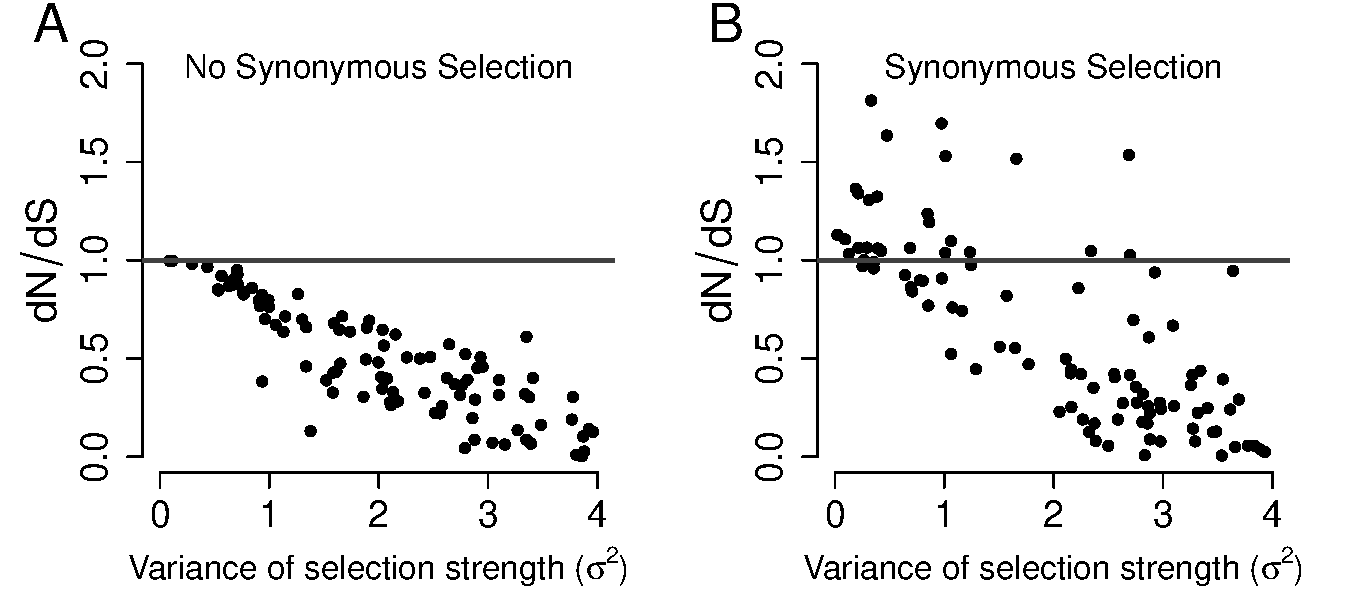
\includegraphics[width=8.7cm]{figures/MainText/dnds_variance.pdf}}
	\caption{\label{dnds_variance} $dN/dS$ decreases in proportion to amino-acid level selection strength. $dN/dS$ is plotted against the $\sigma^2 $ of the simulated distribution of amino-acid scaled selection coefficients. Higher values of $\sigma^2$ indicate larger fitness differences among amino acids, whereas the limiting value of $\sigma^2 = 0$ means that all amino acids have the same fitness. (A) Synonymous codons have equal fitness values ($r^2=0.83$). (B) Synonymous codons have different fitness values ($r^2=0.45$). Importantly, (B), but not (A) shows $dN/dS$ values greater than 1, in spite of the steady-state evolutionary process.}
\end{figure}
		
		
\vspace{2cm}
		
\begin{figure}[htbp]
	\centerline{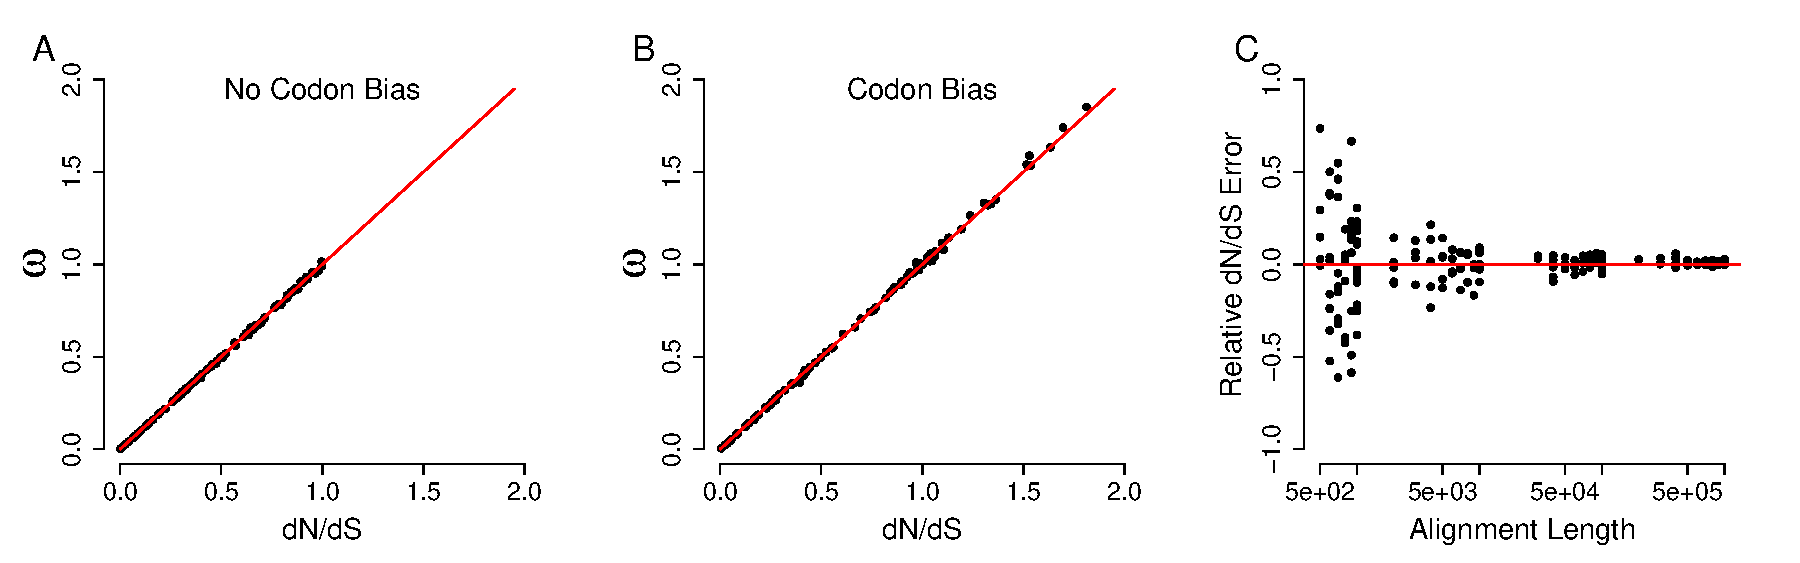
\includegraphics[width=8.7cm]{figures/MainText/regression_convergence.pdf}}
	\caption{\label{reg_conv} Regressions between $dN/dS$ values as calculated from scaled selection coefficients and as inferred using the M0 mechanistic codon model. Each point corresponds to a single simulated alignment. All $\omega$ values shown here were inferred by parameterizing the M0 model with $\kappa$ fixed to its true, simulated value as well as the Fequal codon frequency specification \cite{Yang2006}. The red line in panels (A-B) is the $x=y$ line. (A) Synonymous codons have equal fitness ($r^2=0.997$). (B) Synonymous codons have different fitness values ($r^2=0.992$). (C) Convergence of $\omega$ MLEs to the true $dN/dS$ value. The y-axis indicates the relative error of the maximum likelihood $dN/dS$ estimate, and the x-axis indicates the number of positions in the simulated alignment. As the number of positions, and hence the size of the data set, increases, the maximum likelihood estimates converge to the $dN/dS$ values calculated using equations \eqref{eq:pi_i}-\eqref{eq:dS}. The red line in panel (C) is the line $y=0$, indicating no error.}
\end{figure}
	
\vspace{2cm}
	

\begin{figure}[htbp]
	\centerline{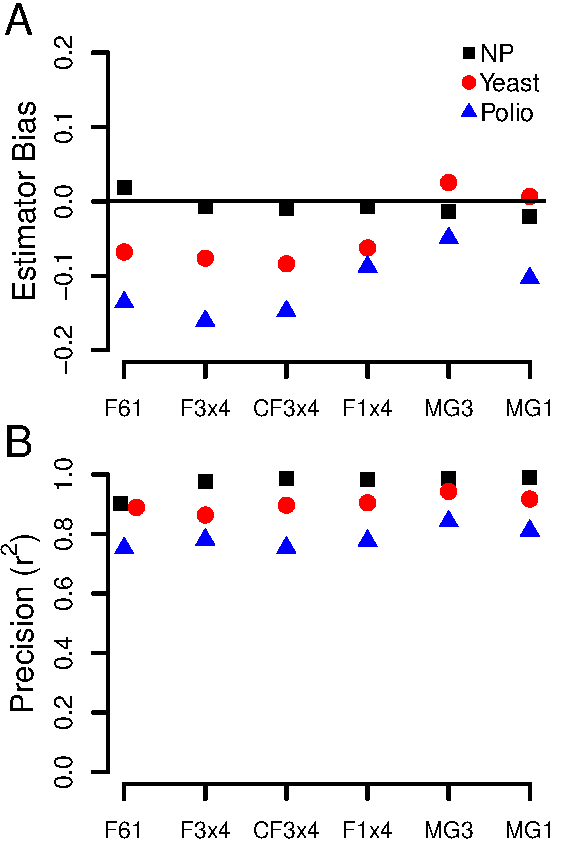
\includegraphics[width=8.7cm]{figures/MainText/nyp_bias_r2.pdf}}
	\caption{\label{nyp_bias_r2} (A) Estimator bias and (B) $r^2$ values between $dN/dS$ and $\omega$ MLEs across M0 codon frequency parameterizations, for each set of nucleotide mutation rates. Note that negative biases indicate $\omega$ values that are, on average, lower than $dN/dS$. All bias and $r^2$ values are highly statistically significant, with all $p < 10^{-12}$. In this figure, we see that $\omega$-based models tend to systematically underestimate $dN/dS$, across all codon frequency parameterizations. Generally, F\protect\xline equal features the least amount of bias, and has very high $r^2$ values for both NP and yeast mutation rates. Although Fequal yields lower $r^2$ values for polio mutation rates than do F61, F3x4, and CF3x4, the latter three estimators also have relatively high biases, demonstrating that they systematically underestimate $dN/dS$. That Ftrue, which assigns codon frequencies to those which would exist in the absence of amino-acid level selection, also underestimates $dN/dS$ implies that codon frequency parameters are ill-suited to accomodate mutation-induced nucleotide compositional bias.}	
\end{figure}

\vspace{2cm}	
	
\begin{table}[htbp]
	\caption {\label{tab:AIC_yeast} Yeast mean($\sigma$) $\Delta$AIC.}
	\begin{tabular}{l c c c}
		\hline\noalign{\smallskip}
		\multicolumn{1}{c}{Frequencies} & k & Empirical $\Delta$AIC & True $\Delta$AIC \\
		\noalign{\smallskip}\hline\noalign{\smallskip}
		Fnuc & 5 & 0 (0)  & 0 (0)  \\ 
		F1x4 & 5 & -3967854.04 (147922.33)  & -3974571.92 (181909.82)  \\ 
		CF3x4 & 11 & -3963057.08 (148227.46)  & -3973790.54 (191530.31)  \\ 
		F3x4 & 11 & -3972768.03 (150045.35)  & -3980424.02 (191521.22)  \\ 
		F61 & 62 & -3955505.20 (148023.84)  & -3974007.80 (191678.03)  \\ 
		\noalign{\smallskip}\hline\noalign{\smallskip} 
	\end{tabular}
\end{table}
\clearpage

	
\section{Supplementary Information}

\vspace{2cm}

\noindent Table S1. Estimator bias between $\omega$ MLEs and the expected, true $dN/dS$ values, for all mutation rates and M0 codon frequency parameterizations examined. Negative bias values indicate that $\omega$ MLEs are, on average, lower than $dN/dS$. All biases are statistically significant, with all $p < 2\times10^{-16}$.
\begin{table}[htbp]
	\begin{tabular}{c c c c c c}
		\hline\noalign{\smallskip}
		Mutation rate & Fnuc & F1x4 & CF3x4 & F3x4 & F61 \\
		\hline\noalign{\smallskip}
		& \multicolumn{5}{c}{Empirical Frequencies}\\
		\cline{2-6}\noalign{\medskip}
		NP & -0.014 & -0.007 & -0.009 & -0.007 & 0.02 \\ 
		Yeast & 0.022 & -0.061 & -0.079 & -0.072 & -0.062 \\ 
		Polio & -0.046 & -0.083 & -0.143 & -0.156 & -0.129 \\ 
		\hline\noalign{\medskip}
		& \multicolumn{5}{c}{True Frequencies}\\
		\cline{2-6}\noalign{\medskip}
		NP & -0.01 & -0.006 & -0.01 & -0.008 & -0.01 \\ 
		Yeast & 0.028 & -0.066 & -0.078 & -0.07 & -0.078 \\ 
		Polio & -0.041 & -0.085 & -0.093 & -0.108 & -0.093 \\ 
		\noalign{\smallskip}\hline\noalign{\smallskip}
	\end{tabular}
\end{table}	

\vspace{2cm}

\noindent Table S2. NYP $r^2$ values between $\omega$ MLEs and $dN/dS$, for all mutation rates and M0 codon frequency parameterizations examined. All $r^2$ values are statistically significant, with all $p < 2\times10^{-16}$.
\begin{table}[htbp]
	\begin{tabular}{c c c c c c}
		\hline\noalign{\smallskip}
		Mutation rate & Fnuc & F1x4 & CF3x4 & F3x4 & F61 \\
		\hline\noalign{\smallskip}
		& \multicolumn{5}{c}{Empirical Frequencies}\\
		\cline{2-6}\noalign{\medskip}
		NP & 0.987 & 0.985 & 0.985 & 0.977 & 0.903 \\ 
		Yeast & 0.937 & 0.919 & 0.909 & 0.876 & 0.902 \\ 
		Polio & 0.870 & 0.796 & 0.777 & 0.800 & 0.770 \\ 
		\hline\noalign{\medskip}
		& \multicolumn{5}{c}{True Frequencies}\\
		\cline{2-6}\noalign{\medskip}
		NP & 0.986 & 0.988 & 0.986 & 0.985 & 0.986 \\ 
		Yeast & 0.954 & 0.868 & 0.836 & 0.814 & 0.834 \\ 
		Polio & 0.929 & 0.763 & 0.735 & 0.765 & 0.736 \\ 
		\noalign{\smallskip}\hline\noalign{\smallskip}
	\end{tabular}
\end{table}	

\vspace{2cm}

\noindent Table S3. NP mean $\Delta$AIC.
\begin{table}[htbp]
	\begin{tabular}{l c c c}
		\hline\noalign{\smallskip}
		\multicolumn{1}{c}{Frequencies} & k & Empirical $\Delta$AIC & True $\Delta$AIC \\
		\noalign{\smallskip}\hline\noalign{\smallskip}
		Fnuc & 5 & 0 (0)  & 0 (0)  \\ 
		F1x4 & 5 & -4110522.59 (29403.83)  & -4113176.42 (18936.59)  \\ 
		CF3x4 & 11 & -4106695.83 (32092.47)  & -4110412.62 (5198.40)  \\ 
		F3x4 & 11 & -4112103.30 (50194.48)  & -4113684.34 (28635.18)  \\ 
		F61 & 62 & -4096741.43 (65475.10)  & -4110482.75 (5316.52)  \\ 
		\noalign{\smallskip}\hline\noalign{\smallskip} 
	\end{tabular}
\end{table}

\vspace{2cm}

\noindent Table S4. Polio mean $\Delta$AIC.
\begin{table}[htbp]
	\begin{tabular}{l c c c}
		\hline\noalign{\smallskip}
		\multicolumn{1}{c}{Frequencies} & k & Empirical $\Delta$AIC & True $\Delta$AIC \\
		\noalign{\smallskip}\hline\noalign{\smallskip}
		Fnuc & 5 & 0 (0)  & 0 (0)  \\ 
		F1x4 & 5 & -3535535.65 (256147.28)  & -3548685.06 (291042.26)  \\ 
		CF3x4 & 11 & -3528315.59 (244833.08)  & -3543917.87 (294076.66)  \\ 
		F3x4 & 11 & -3539604.01 (253746.00)  & -3555805.19 (302106.86)  \\ 
		F61 & 62 & -3520641.22 (238395.84)  & -3543716.83 (293919.71)  \\ 
		\noalign{\smallskip}\hline\noalign{\smallskip} 
	\end{tabular}
\end{table}


\newpage

\begin{landscape}
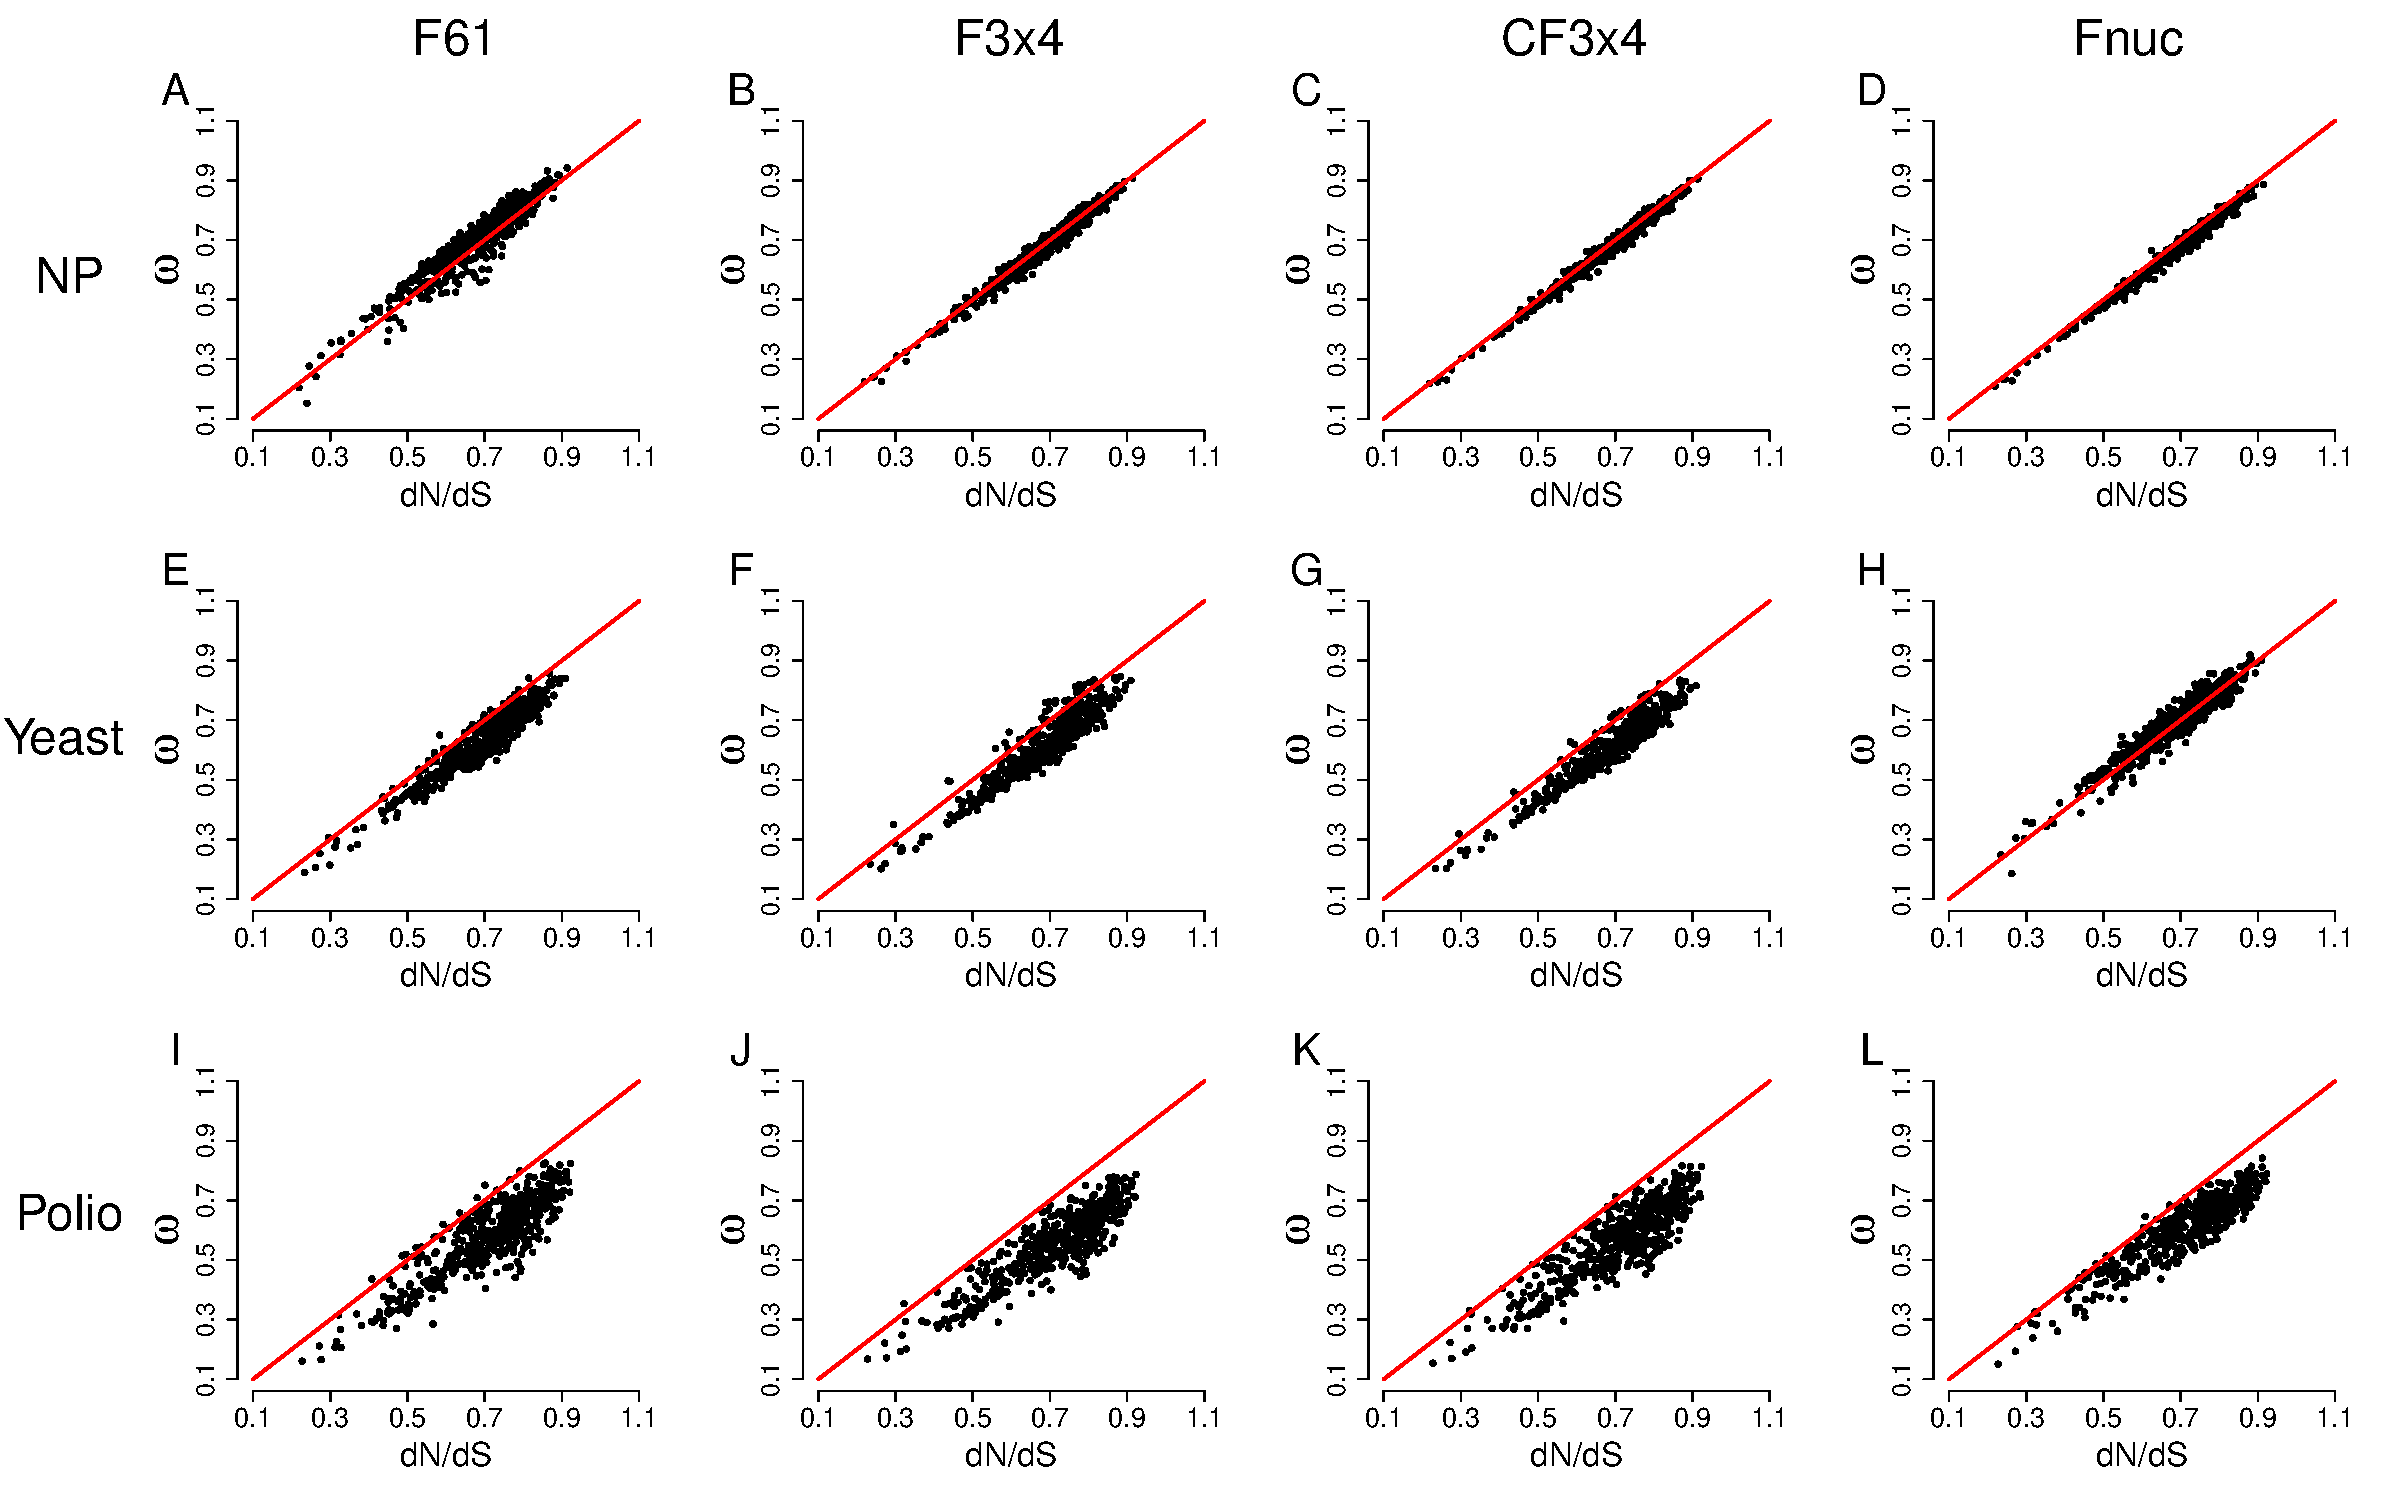
\includegraphics[width=9in]{figures/SI/nyp_datafreqs.pdf}
\vspace{0.5cm}

\noindent Figure S1. REWRITE: Regression plots for $\omega$ MLEs versus $dN/dS$ values computed from scaled selection coefficients, for each set of nucleotide mutation rates and all M0 codon frequency parameterizations. Each point represents a single simulated alignment, and the red lines correspond to $x=y$. (A) Simulations which assigned equal fitness values to synonymous codons. (B) Simulations which allowed different fitness values among synonymous codons.
\end{landscape}

\begin{landscape}
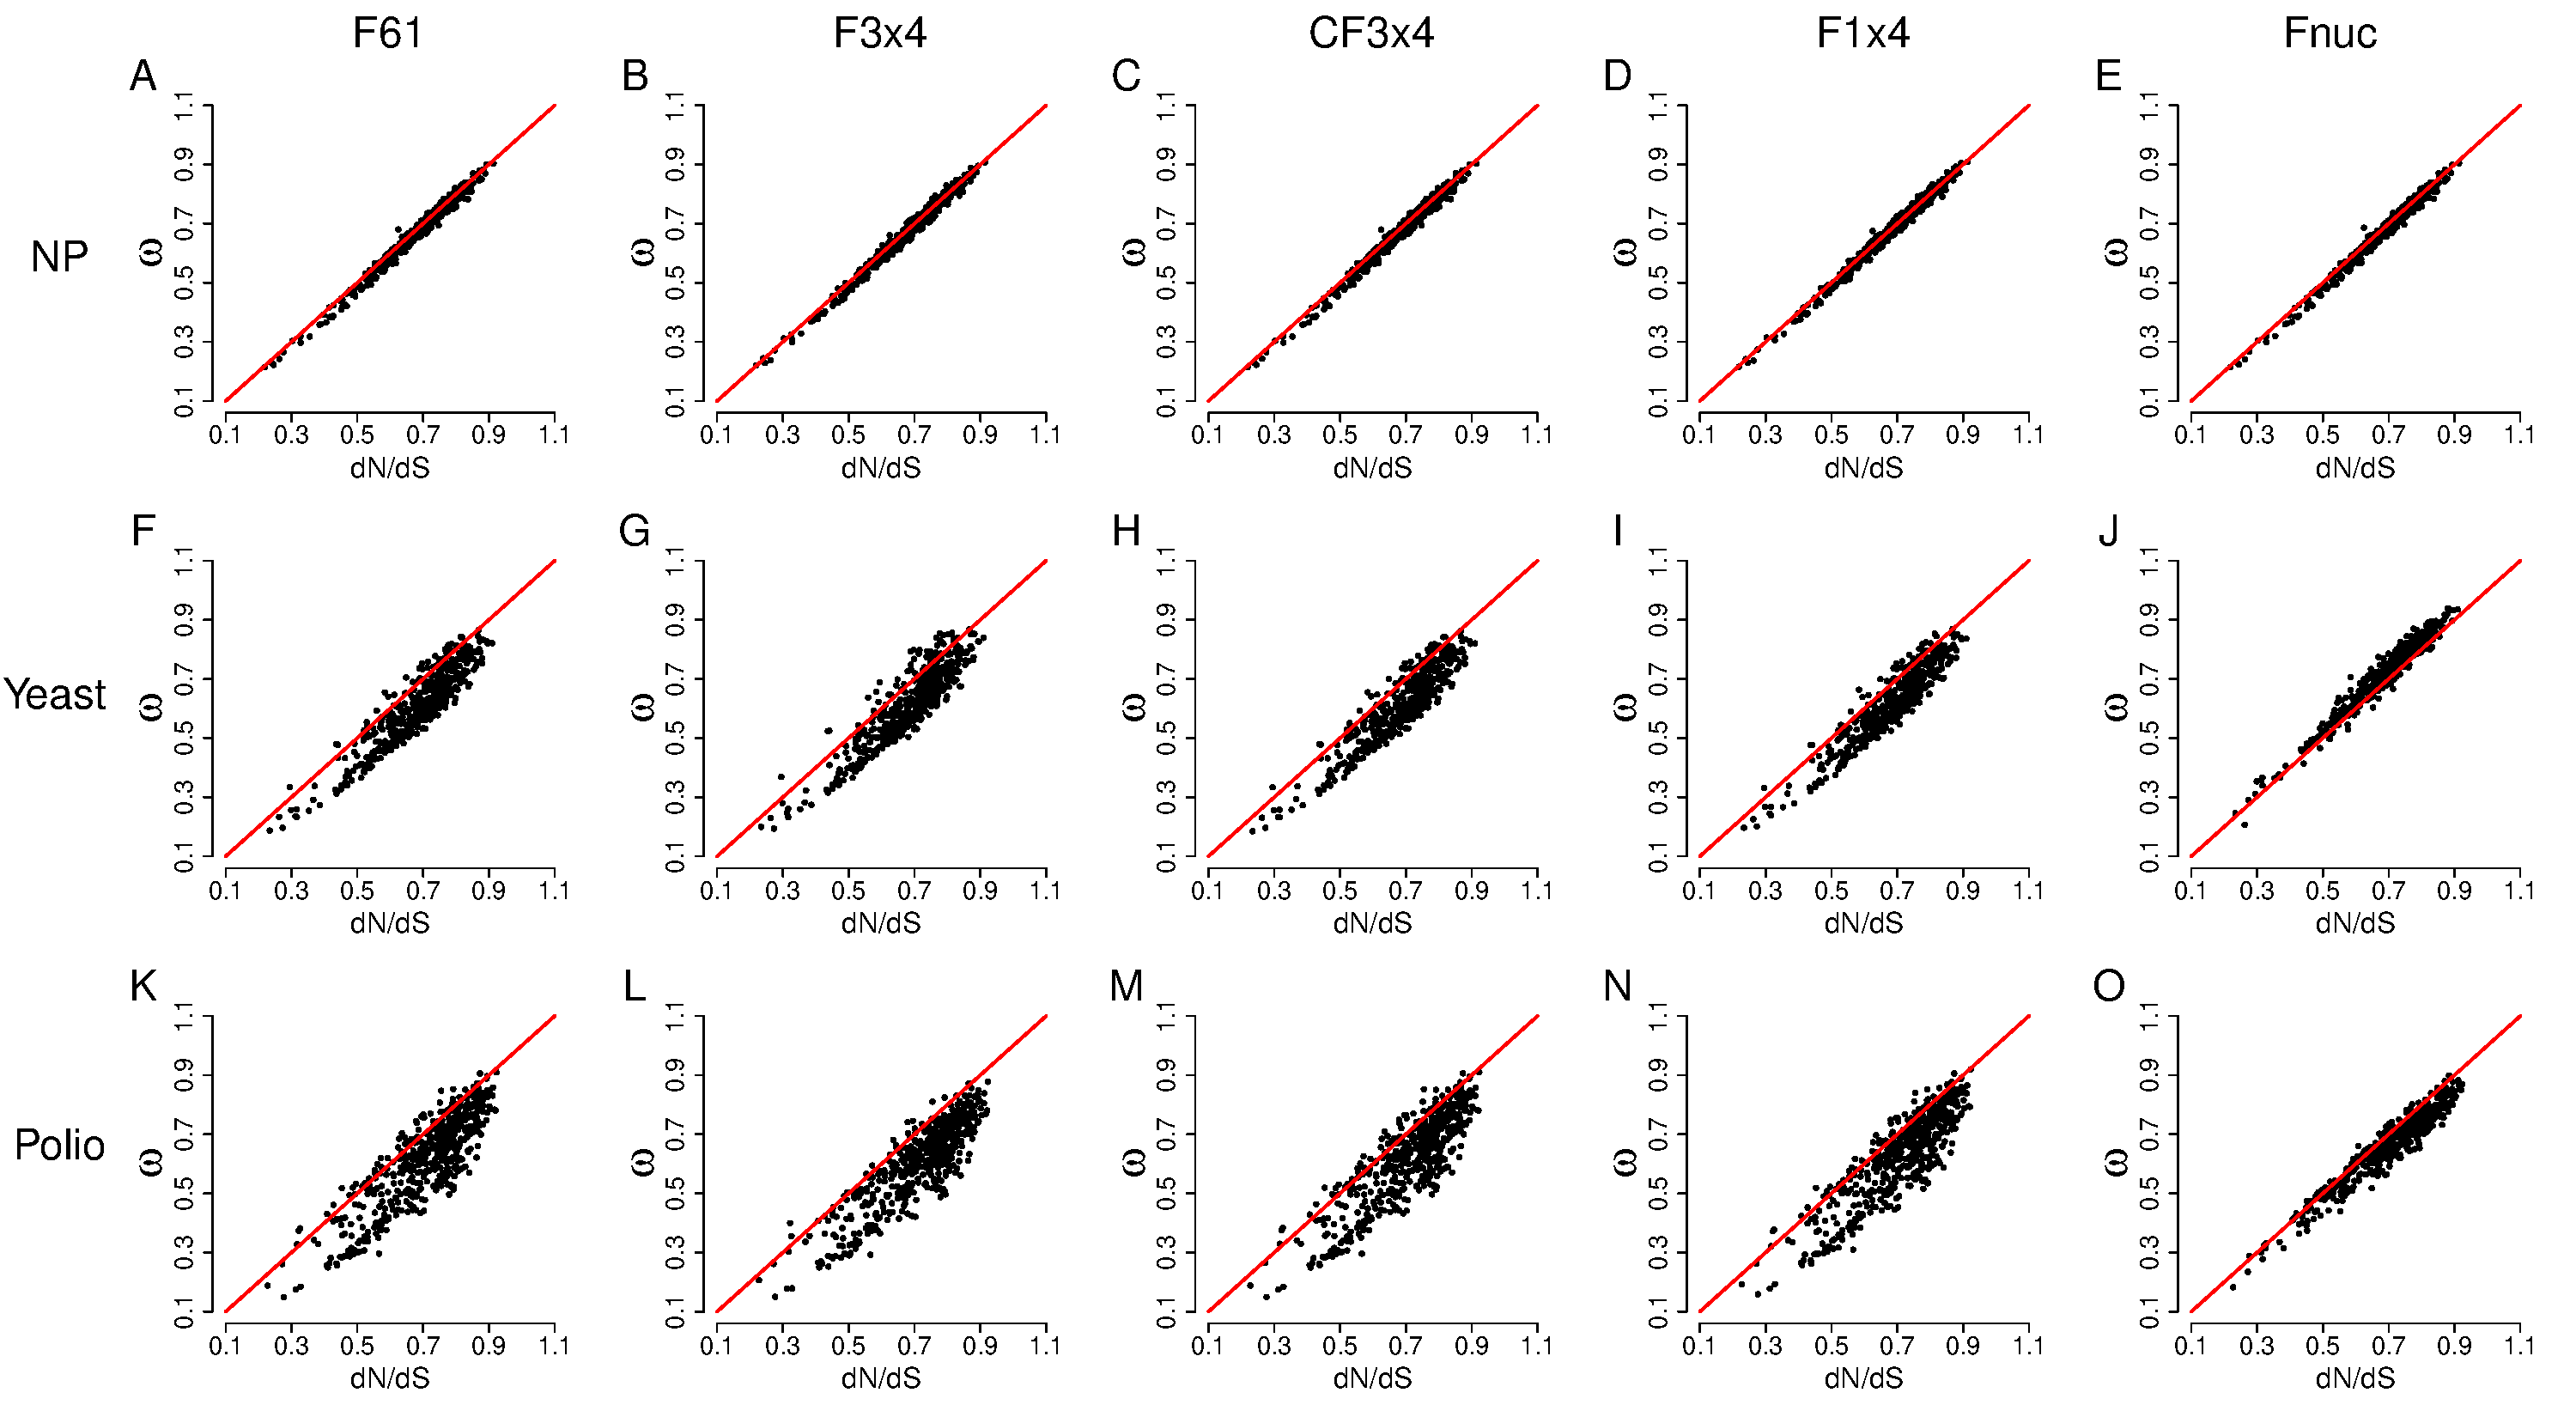
\includegraphics[width=9in]{figures/SI/nyp_truefreqs.pdf}
\vspace{0.5cm}

\noindent Figure S2. REWRITE: Regression plots for $\omega$ MLEs versus $dN/dS$ values computed from scaled selection coefficients, for each set of nucleotide mutation rates and all M0 codon frequency parameterizations. Each point represents a single simulated alignment, and the red lines correspond to $x=y$. (A) Simulations which assigned equal fitness values to synonymous codons. (B) Simulations which allowed different fitness values among synonymous codons.
\end{landscape}
	
\end{document}

